\chapter{Avaliação de Resultados}
\label{ch:resultados}

O Capítulo~\ref{ch:resultados} apresenta os resultados obtidos. A
Secção~\ref{sec:res-tec} reúne as métricas técnicas dos três casos de
estudo. A Secção~\ref{sec:res-rankings} apresenta os rankings
produzidos pelos três algoritmos. A Secção~\ref{sec:res-correlacoes}
quantifica formalmente a concordância entre algoritmos via Spearman
$\rho$ e Kendall $\tau_b$ (resposta a RQ1 e RQ2). A
Secção~\ref{sec:res-consolidada} consolida a comparação entre
projetos. A Secção~\ref{sec:discussao} discute as observações
principais (resposta a RQ3). A Secção~\ref{sec:ameacas} enuncia
formalmente as ameaças à validade.

\noindent\textbf{Conceitos-chave:} resultados técnicos; resultados
analíticos; correlação de ranks; convergência \emph{a priori};
divergência informativa; ameaças à validade.

% ---------------------------------------------------------------------------
\section{Resultados Técnicos}
\label{sec:res-tec}

Esta secção sintetiza as métricas estruturais obtidas em cada caso
de estudo, evidenciando a escalabilidade do \emph{pipeline} e o grau
de acoplamento detetado em cada projeto.

\subsection{Síntese Quantitativa}
\label{sec:res-sintese}

A Tabela~\ref{tab:sintese-quant} resume as principais métricas
obtidas pelo \emph{pipeline} \emph{ReqGraph} nos três casos de
estudo. As contagens reportadas distinguem (i) o número total de
requisitos \emph{mapeados} no ficheiro \code{mapeamento.py} e (ii)
o número de requisitos \emph{efetivamente presentes} no
\code{req\_graph.json} (\ie\ com pelo menos uma aresta incidente). A
distinção é metodologicamente relevante: requisitos isolados
(\emph{singletons}) não contribuem para o ranking estrutural --- são
discutidos como \emph{ameaça à validade interna} na
Secção~\ref{sec:ameacas}.

\begin{table}[ht]
    \centering
    \caption{Síntese quantitativa dos três casos de estudo.
    \emph{Densidade} é calculada como $|E| / (n(n-1))$ sobre
    requisitos com arestas.}
    \label{tab:sintese-quant}
    \begin{tabular}{@{}l r r r@{}}
        \toprule
        \textbf{Métrica} & \textbf{CPython \emph{stdlib}} & \textbf{Flask} & \textbf{\emph{scikit-learn}} \\
        \midrule
        Ficheiros analisados                & 2     & 3     & 4 \\
        Funções/métodos detetados           & 298   & 125   & 210 \\
        Arestas no \emph{Call Graph}        & 130   & 47    & 80 \\
        \textbf{Requisitos mapeados (\code{mapeamento.py})}  & 10    & 13    & 9 \\
        \textbf{Requisitos com arestas no Grafo de Requisitos} & 9     & 7     & 8 \\
        Requisitos isolados (\emph{singletons})              & 1     & 6     & 1 \\
        Arestas no Grafo de Requisitos      & 9     & 11    & 17 \\
        Densidade $|E|/(n(n-1))$            & $0{,}125$ & $0{,}262$ & $0{,}304$ \\
        Resultado da execução               & Passou & Passou & Passou \\
        \bottomrule
    \end{tabular}
\end{table}

\paragraph{Discussão das contagens.} Observa-se que o número de
funções analisadas não cresce monotonicamente com a complexidade
percebida (o \code{argparse} da \emph{stdlib} tem mais funções do
que o \code{app.py} do Flask), mas o número de arestas no Grafo de
Requisitos cresce de forma quase monotónica --- passando de $9$
(CPython) para $11$ (Flask) e $17$ (\emph{scikit-learn}). Esta
métrica é, portanto, mais informativa sobre o acoplamento
arquitetural do que a contagem bruta de funções.

\paragraph{Requisitos isolados.} O caso \textbf{Flask} merece
atenção: dos $13$ requisitos mapeados, apenas $7$ aparecem no Grafo
de Requisitos. Os $6$ requisitos isolados ---
\req{REQ\_BLUEPRINTS}, \req{REQ\_CLI\_DISCOVERY},
\req{REQ\_CLI\_TYPES}, \req{REQ\_STATIC\_FILES}, \req{REQ\_TEMPLATING}
e \req{REQ\_TESTING} --- correspondem a funções que, dentro dos três
ficheiros analisados, não invocam funções de outros requisitos nem
são invocadas por elas. Esta observação é
\emph{informativa}: revela que parte significativa da arquitetura do
Flask referenciada no mapeamento está implementada \emph{fora} dos
ficheiros analisados (e.g., a \emph{templating engine} reside em
\code{jinja2}, externa ao corpus). Trata-se de uma limitação direta
da estratégia de seleção de ficheiros (Secção~\ref{sec:protocolo}) e
é endereçada como ameaça à \emph{external validity}
(Secção~\ref{sec:ameacas}).

\paragraph{Densidade.} Os valores de densidade $0{,}125$, $0{,}262$
e $0{,}304$ correspondem ao crescimento esperado de acoplamento
arquitetural. Importa, contudo, ressalvar (\cf\ \citealt{newman2010}):
em grafos com poucas dezenas de vértices, a densidade é uma métrica
\emph{volátil} --- pequenas variações no mapeamento podem deslocá-la
significativamente. Por essa razão, na Secção~\ref{sec:discussao}
discutem-se também as variações de \emph{clustering coefficient} e
de presença de ciclos como métricas complementares.

\subsection{Caso Simples --- CPython \emph{stdlib}}
\label{sec:res-stdlib}

Foram analisados os módulos \code{argparse.py} (\emph{parsing} de
argumentos) e \code{http/server.py} (servidor HTTP simples). O
mapeamento associa $298$ funções a $10$ requisitos de domínio, dos
quais $9$ aparecem no Grafo de Requisitos. O grafo resultante
apresenta apenas $9$ arestas, sem ciclos, e pode ser sintetizado
pelas seguintes adjacências:

\begin{lstlisting}[language=json, caption={Adjacências do Grafo de Requisitos --- CPython \emph{stdlib}.},label={lst:stdlib-json}]
{
  "REQ_ACTIONS":        ["REQ_CONFIGURATION", "REQ_FORMATTING", "REQ_VALIDATION"],
  "REQ_ERROR_HANDLING": ["REQ_FORMATTING"],
  "REQ_FORMATTING":     ["REQ_ERROR_HANDLING"],
  "REQ_HTTP_HANDLER":   ["REQ_HTTP_CONTENT", "REQ_HTTP_LOGGING"],
  "REQ_PARSING":        ["REQ_ERROR_HANDLING", "REQ_VALIDATION"]
}
\end{lstlisting}

O grafo divide-se claramente em dois sub-sistemas independentes
(\emph{parsing}/\code{argparse} \emph{vs.\ }HTTP), confirmando o
baixo acoplamento esperado de módulos da biblioteca padrão. O único
ciclo identificado é o par
\req{REQ\_FORMATTING}~$\leftrightarrow$~\req{REQ\_ERROR\_HANDLING},
refletindo a coexistência das funções \code{format\_help} e
\code{error}, que se chamam mutuamente.

\begin{figure}[ht]
    \centering
    
\includegraphics[width=0.75\linewidth]{req_graph_simples_stdlib.png}
    \caption{Grafo de Requisitos: CPython \emph{stdlib}. Note-se a
    divisão clara em dois sub-sistemas independentes
    (\emph{parsing}/\code{argparse} \emph{vs.\ }HTTP) e o ciclo
    \req{FORMATTING}~$\leftrightarrow$~\req{ERROR\_HANDLING}.}
    \label{fig:req-stdlib}
\end{figure}

\subsection{Caso Intermediário --- Flask}
\label{sec:res-flask}

Foram analisados \code{app.py}, \code{cli.py} e \code{blueprints.py},
perfazendo $125$ funções mapeadas em $13$ requisitos, dos quais
\textbf{apenas $7$ aparecem no Grafo de Requisitos} (ver discussão
em Secção~\ref{sec:res-sintese}). O Grafo de Requisitos contém
$11$ arestas e --- diferentemente do caso anterior --- apresenta
\textbf{fortes relações cíclicas}:

\begin{lstlisting}[language=json, caption={Adjacências do Grafo de Requisitos --- Flask.},label={lst:flask-json}]
{
  "REQ_APP_CORE":         ["REQ_CLI_COMMANDS", "REQ_CLI_FRAMEWORK", "REQ_CONTEXT"],
  "REQ_CLI_FRAMEWORK":    ["REQ_CONTEXT"],
  "REQ_CONTEXT":          ["REQ_REQUEST_HANDLING"],
  "REQ_ERROR_HANDLING":   ["REQ_REQUEST_HANDLING"],
  "REQ_REQUEST_HANDLING": ["REQ_CONTEXT", "REQ_ERROR_HANDLING", "REQ_ROUTING"],
  "REQ_ROUTING":          ["REQ_ERROR_HANDLING", "REQ_REQUEST_HANDLING"]
}
\end{lstlisting}

O ciclo
\req{REQUEST\_HANDLING} $\leftrightarrow$ \req{CONTEXT} $\leftrightarrow$
\req{ROUTING} $\leftrightarrow$ \req{ERROR\_HANDLING} evidencia que
estas quatro responsabilidades estão estreitamente acopladas, o que
é coerente com a arquitetura \emph{middleware} do Flask, onde o
ciclo de vida de uma requisição obriga à coordenação entre
\emph{dispatcher}, contexto de aplicação e tratamento de exceções.

Na Figura~\ref{fig:req-flask}, \textbf{as cores atribuídas aos
vértices identificam o ficheiro-fonte do projeto a que cada
requisito pertence} (azul para \code{app.py}, verde para
\code{cli.py}, laranja para \code{blueprints.py}), permitindo
perceber visualmente como o acoplamento atravessa os módulos. As
cores das arestas seguem a cor do vértice de origem, facilitando a
leitura das cadeias de dependência.

\begin{figure}[ht]
    \centering
    
\includegraphics[width=0.75\linewidth]{req_graph_medio_flask.png}
    \caption{Grafo de Requisitos: Flask. O ciclo
    \req{REQUEST\_HANDLING}~$\leftrightarrow$~\req{CONTEXT}~$\leftrightarrow$~\req{ROUTING}~$\leftrightarrow$~\req{ERROR\_HANDLING}
    evidencia o forte acoplamento típico do \emph{middleware}.}
    \label{fig:req-flask}
\end{figure}

\subsection{Caso Complexo --- \emph{scikit-learn}}
\label{sec:res-sklearn}

Foram analisados \code{pipeline.py},
\code{linear\_model/\_base.py}, \code{linear\_model/\_logistic.py}
e \code{tree/\_classes.py}, contabilizando $210$ funções mapeadas
em $9$ requisitos, dos quais $8$ aparecem no Grafo de Requisitos
(\req{REQ\_SPARSE} fica isolado). O Grafo de Requisitos resultante
é o \textbf{mais denso} dos três casos ($17$ arestas, densidade
$0{,}304$), refletindo o elevado grau de orquestração interna do
\emph{framework}:

\begin{lstlisting}[language=json, caption={Adjacências do Grafo de Requisitos --- \emph{scikit-learn}.},label={lst:sklearn-json}]
{
  "REQ_DECISION_TREE":       ["REQ_SKLEARN_TAGS"],
  "REQ_FEATURE_UNION":       ["REQ_PIPELINE"],
  "REQ_LOGISTIC_REGRESSION": ["REQ_PIPELINE_PREDICT"],
  "REQ_PIPELINE":            ["REQ_LOGISTIC_REGRESSION", "REQ_PIPELINE_PREDICT", "REQ_SKLEARN_TAGS"],
  "REQ_PIPELINE_FIT":        ["REQ_DECISION_TREE", "REQ_FEATURE_UNION", "REQ_LINEAR_MODEL", "REQ_LOGISTIC_REGRESSION", "REQ_PIPELINE"],
  "REQ_PIPELINE_PREDICT":    ["REQ_DECISION_TREE", "REQ_FEATURE_UNION", "REQ_LINEAR_MODEL", "REQ_LOGISTIC_REGRESSION", "REQ_PIPELINE"],
  "REQ_SKLEARN_TAGS":        ["REQ_PIPELINE"]
}
\end{lstlisting}

\req{REQ\_PIPELINE\_FIT} e \req{REQ\_PIPELINE\_PREDICT} conectam-se
cada um a cinco outros requisitos, confirmando o seu papel de
\textbf{orquestradores centrais}. \req{REQ\_PIPELINE} recebe arestas
de quatro requisitos distintos, sendo a \textbf{autoridade
dominante} do sistema.

\begin{figure}[ht]
    \centering
    
\includegraphics[width=0.85\linewidth]{req_graph_complexo_sklearn.png}
    \caption{Grafo de Requisitos: \emph{scikit-learn}. O caso mais
    denso (17 arestas) reflete a orquestração interna do
    \emph{framework}: \req{REQ\_PIPELINE\_FIT} e
    \req{REQ\_PIPELINE\_PREDICT} conectam-se cada um a cinco outros
    requisitos.}
    \label{fig:req-sklearn}
\end{figure}

% ---------------------------------------------------------------------------
\section{Rankings produzidos pelos três algoritmos}
\label{sec:res-rankings}

Esta secção apresenta os rankings produzidos pelo PageRank, HITS e
SALSA para cada caso de estudo, interpretando os \emph{scores} à luz
da arquitetura conhecida dos projetos.

\subsection{Caso Simples --- Rankings para o CPython \emph{stdlib}}
\label{sec:res-stdlib-rank}

A Tabela~\ref{tab:top3-stdlib} reúne os três primeiros requisitos
identificados por cada algoritmo. \textbf{Os valores entre
parênteses correspondem ao \emph{score} numérico} atribuído pelo
respetivo algoritmo --- para o PageRank, são probabilidades
estacionárias (somam $1$ no total do grafo); para o HITS, são
componentes de vetores normalizados (norma euclidiana unitária);
para o SALSA, são componentes de vetores normalizados por soma
unitária (cada vetor --- \emph{authority} ou \emph{hub} --- soma
$1$). \emph{Scores} mais elevados indicam maior centralidade segundo
o critério do algoritmo.

\begin{table}[ht]
    \centering
    \caption{\emph{Top-3} por algoritmo: CPython \emph{stdlib}.}
    \label{tab:top3-stdlib}
    \footnotesize
    \begin{tabular}{@{}l l l l@{}}
        \toprule
        \textbf{Algoritmo} & \textbf{1.º} & \textbf{2.º} & \textbf{3.º} \\
        \midrule
        \textbf{PageRank}              & \req{REQ\_ERROR\_HANDLING} ($0{,}337$) & \req{REQ\_FORMATTING} ($0{,}334$) & \req{REQ\_VALIDATION} ($0{,}064$) \\
        \textbf{HITS --- Authority}    & \req{REQ\_VALIDATION} ($0{,}338$)      & \req{REQ\_FORMATTING} ($0{,}280$) & \req{REQ\_CONFIGURATION} ($0{,}209$) \\
        \textbf{HITS --- Hub}          & \req{REQ\_ACTIONS} ($0{,}462$)         & \req{REQ\_PARSING} ($0{,}285$)    & \req{REQ\_ERROR\_HANDLING} ($0{,}156$) \\
        \textbf{SALSA --- Authority}   & \req{REQ\_HTTP\_CONTENT} ($0{,}167$)   & \req{REQ\_HTTP\_LOGGING} ($0{,}167$) & \req{REQ\_ERROR\_HANDLING} ($0{,}167$) \\
        \textbf{SALSA --- Hub}         & \req{REQ\_HTTP\_HANDLER} ($0{,}200$)   & \req{REQ\_ERROR\_HANDLING} ($0{,}200$) & \req{REQ\_ACTIONS} ($0{,}200$) \\
        \bottomrule
    \end{tabular}
\end{table}

O PageRank identifica \req{REQ\_ERROR\_HANDLING} como o requisito
mais crítico, concentrando $0{,}337$ da probabilidade estacionária
--- ou seja, \textbf{um caminhante aleatório que percorra o grafo
durante muito tempo passará cerca de $33{,}7\%$ do tempo nesse
vértice}. Esta é a interpretação direta da ``massa de probabilidade''
a que o PageRank dá origem: cada \emph{score} indica que fração do
tempo um passeio aleatório de longa duração visita aquele vértice.
\req{REQ\_FORMATTING} segue muito de perto ($0{,}334$). Esta dupla
decorre do ciclo
\req{FORMATTING} $\leftrightarrow$ \req{ERROR\_HANDLING}, que faz a
probabilidade acumular-se nesses dois vértices via \emph{random
walk}. O HITS distingue claramente os papéis: \req{REQ\_ACTIONS} e
\req{REQ\_PARSING} são \emph{hubs} (consomem muitas dependências),
enquanto \req{REQ\_VALIDATION}, \req{REQ\_FORMATTING} e
\req{REQ\_CONFIGURATION} são \emph{authorities} (são consumidos por
muitos). O \textbf{SALSA}, devido à sua normalização local, atribui
\emph{scores} idênticos a todos os vértices com arestas ---
comportamento esperado em grafos com graus pouco diferenciados
(\cf\ \citealt{lempel2001}).

\begin{figure}[ht]
    \centering
    
\includegraphics[width=0.85\linewidth]{ranking_results_simples_stdlib.png}
    \caption{Rankings produzidos pelos três algoritmos para o caso
    CPython \emph{stdlib}.}
    \label{fig:rankings-stdlib}
\end{figure}

\subsection{Caso Intermediário --- Rankings para o Flask}
\label{sec:res-flask-rank}

A Tabela~\ref{tab:top3-flask} apresenta os \emph{top-3} do caso
médio. Para os algoritmos SALSA, ``uniforme entre 6 requisitos''
significa que seis vértices receberam o mesmo \emph{score}
($1/6 \approx 0{,}167$); os requisitos isolados receberam \emph{score}
zero (não contam para o top).

\begin{table}[ht]
    \centering
    \caption{\emph{Top-3} por algoritmo: Flask.}
    \label{tab:top3-flask}
    \footnotesize
    \begin{tabular}{@{}l l l l@{}}
        \toprule
        \textbf{Algoritmo} & \textbf{1.º} & \textbf{2.º} & \textbf{3.º} \\
        \midrule
        \textbf{PageRank}              & \req{REQ\_REQUEST\_HANDLING} ($0{,}400$) & \req{REQ\_ERROR\_HANDLING} ($0{,}198$) & \req{REQ\_CONTEXT} ($0{,}174$) \\
        \textbf{HITS --- Authority}    & \req{REQ\_CONTEXT} ($0{,}318$)         & \req{REQ\_ERROR\_HANDLING} ($0{,}204$) & \req{REQ\_ROUTING} ($0{,}137$) \\
        \textbf{HITS --- Hub}          & \req{REQ\_REQUEST\_HANDLING} ($0{,}319$) & \req{REQ\_APP\_CORE} ($0{,}264$)     & \req{REQ\_CLI\_FRAMEWORK} ($0{,}154$) \\
        \textbf{SALSA --- Authority}   & \multicolumn{3}{c}{\emph{uniforme} a $0{,}167$ entre 6 requisitos com arestas} \\
        \textbf{SALSA --- Hub}         & \multicolumn{3}{c}{\emph{uniforme} a $0{,}167$ entre 6 requisitos com arestas} \\
        \bottomrule
    \end{tabular}
\end{table}

\req{REQ\_REQUEST\_HANDLING} emerge como o vértice central segundo o
PageRank, com $40\%$ da probabilidade estacionária --- um valor
anormalmente elevado que reflete a sua posição em três arestas de
entrada e três de saída, todas dentro do ciclo principal. O HITS
divide o protagonismo: \req{REQ\_REQUEST\_HANDLING} é simultaneamente
\emph{hub} e \emph{authority} (acoplamento bidirecional típico do
\emph{middleware}), enquanto \req{REQ\_CONTEXT} lidera as
\emph{authorities} puras. O SALSA produziu uma \textbf{distribuição
praticamente uniforme}, alinhada com a propriedade demonstrada por
\citet{lempel2001}: em grafos com graus pouco diferenciados, o
\emph{score} converge para uma constante por classe de equivalência
de grau.

\begin{figure}[ht]
    \centering
    
\includegraphics[width=0.85\linewidth]{ranking_results_medio_flask.png}
    \caption{Rankings produzidos pelos três algoritmos para o caso
    Flask.}
    \label{fig:rankings-flask}
\end{figure}

\subsection{Caso Complexo --- Rankings para \emph{scikit-learn}}
\label{sec:res-sklearn-rank}

A Tabela~\ref{tab:top3-sklearn} apresenta o \emph{top-3} do caso
mais complexo.

\begin{table}[ht]
    \centering
    \caption{\emph{Top-3} por algoritmo: \emph{scikit-learn}.}
    \label{tab:top3-sklearn}
    \footnotesize
    \begin{tabular}{@{}l l l l@{}}
        \toprule
        \textbf{Algoritmo} & \textbf{1.º} & \textbf{2.º} & \textbf{3.º} \\
        \midrule
        \textbf{PageRank}              & \req{REQ\_PIPELINE} ($0{,}257$)        & \req{REQ\_PIPELINE\_PREDICT} ($0{,}218$) & \req{REQ\_SKLEARN\_TAGS} ($0{,}156$) \\
        \textbf{HITS --- Authority}    & \req{REQ\_PIPELINE} ($0{,}217$)        & \req{REQ\_LOGISTIC\_REGRESSION} ($0{,}200$) & \req{REQ\_DECISION\_TREE} ($0{,}177$) \\
        \textbf{HITS --- Hub}          & \req{REQ\_PIPELINE\_PREDICT} ($0{,}360$) & \req{REQ\_PIPELINE\_FIT} ($0{,}360$)      & \req{REQ\_PIPELINE} ($0{,}096$) \\
        \textbf{SALSA --- Authority}   & \multicolumn{3}{c}{\emph{uniforme} a $0{,}143$ entre 7 requisitos com arestas} \\
        \textbf{SALSA --- Hub}         & \multicolumn{3}{c}{\emph{uniforme} a $0{,}143$ entre 7 requisitos com arestas} \\
        \bottomrule
    \end{tabular}
\end{table}

PageRank e HITS coincidem na identificação de \req{REQ\_PIPELINE}
como o requisito mais central: o PageRank atribui-lhe o \emph{score}
mais elevado ($0{,}257$) e o HITS classifica-o como a
\emph{authority} dominante ($0{,}217$). O HITS identifica
adicionalmente \req{REQ\_PIPELINE\_PREDICT} e \req{REQ\_PIPELINE\_FIT}
como co-líderes dos \emph{hubs} com \emph{scores} idênticos
($0{,}360$) --- refletindo a sua simetria estrutural (ambos invocam
exatamente os mesmos cinco requisitos). O SALSA volta a produzir uma
distribuição uniforme entre os vértices com arestas, indicando que,
neste corpus, não há vértices destacados pelas suas frações de grau.

\begin{figure}[ht]
    \centering
    
\includegraphics[width=0.85\linewidth]{ranking_results_complexo_sklearn.png}
    \caption{Rankings produzidos pelos três algoritmos para o caso
    \emph{scikit-learn}.}
    \label{fig:rankings-sklearn}
\end{figure}

% ---------------------------------------------------------------------------
\section{Correlações Spearman e Kendall entre Rankings}
\label{sec:res-correlacoes}

Para responder formalmente a \textbf{RQ1} (em que medida os
algoritmos concordam) e a \textbf{RQ2} (como a concordância varia
com as propriedades estruturais), calcularam-se os coeficientes de
correlação de Spearman ($\rho$) e Kendall ($\tau_b$) entre cada par
de algoritmos, em cada caso de estudo. Os valores foram produzidos
pelo \emph{script} \code{compute\_rank\_correlations.py} e estão
sintetizados na Tabela~\ref{tab:correlacoes}. Em
\colorbox{NoteBg}{realçado} indica-se cada par que satisfaz o
critério \emph{a priori} de \textbf{convergência forte}
(Secção~\ref{sec:metricas}: $\rho \geq 0{,}7$ \emph{e}
$\tau_b \geq 0{,}55$).

\begin{table}[ht]
    \centering
    \caption{Coeficientes de correlação de ranks (Spearman $\rho$,
    Kendall $\tau_b$) entre cada par de algoritmos, por caso de
    estudo. \emph{Top-1} indica se o requisito \emph{top-1} coincide.}
    \label{tab:correlacoes}
    \footnotesize
    \begin{tabular}{@{}l r r c r r c r r c@{}}
        \toprule
        & \multicolumn{3}{c}{\textbf{CPython \emph{stdlib}}}
        & \multicolumn{3}{c}{\textbf{Flask}}
        & \multicolumn{3}{c}{\textbf{\emph{scikit-learn}}} \\
        \cmidrule(lr){2-4}\cmidrule(lr){5-7}\cmidrule(lr){8-10}
        \textbf{Par} & $\rho$ & $\tau_b$ & T1 & $\rho$ & $\tau_b$ & T1 & $\rho$ & $\tau_b$ & T1 \\
        \midrule
        PR vs HITS-auth      & $0{,}65$ & $0{,}49$ & \texttimes & $0{,}60$ & $0{,}53$ & \texttimes & $0{,}39$ & $0{,}33$ & \checkmark \\
        PR vs HITS-hub       & $-0{,}15$ & $-0{,}03$ & \texttimes & $0{,}08$ & $0{,}00$ & \checkmark & $0{,}24$ & $0{,}24$ & \texttimes \\
        \rowcolor{NoteBg}
        PR vs SALSA-auth     & $0{,}84$ & $0{,}75$ & \texttimes & $0{,}62$ & $0{,}55$ & \texttimes & $0{,}59$ & $0{,}53$ & \texttimes \\
        PR vs SALSA-hub      & $-0{,}18$ & $-0{,}16$ & \texttimes & $0{,}31$ & $0{,}27$ & \texttimes & $0{,}25$ & $0{,}23$ & \texttimes \\
        HITS-auth vs SALSA-auth & $0{,}60$ & $0{,}55$ & \texttimes & $0{,}64$ & $0{,}58$ & \texttimes & $0{,}60$ & $0{,}54$ & \texttimes \\
        \rowcolor{NoteBg}
        HITS-hub vs SALSA-hub & $0{,}76$ & $0{,}70$ & \texttimes & $0{,}62$ & $0{,}56$ & \texttimes & $0{,}59$ & $0{,}53$ & \texttimes \\
        \bottomrule
    \end{tabular}
\end{table}

\paragraph{Leitura por caso.} No \textbf{CPython \emph{stdlib}},
dois pares satisfazem o critério de convergência forte:
PR\,$\leftrightarrow$\,SALSA-auth ($\rho=0{,}84$, $\tau_b=0{,}75$) e
HITS-hub\,$\leftrightarrow$\,SALSA-hub ($\rho=0{,}76$, $\tau_b=0{,}70$).
Os \emph{top-1}, contudo, são diferentes: o PageRank captura o
ciclo \req{ERROR\_HANDLING}$\leftrightarrow$\req{FORMATTING} via
massa estacionária, enquanto o SALSA reparte uniformemente.

No \textbf{Flask}, \emph{nenhum par satisfaz o critério forte}; o
único \emph{top-1 match} ocorre entre PR e HITS-hub
(\req{REQ\_REQUEST\_HANDLING}), num par que paradoxalmente tem
$\rho = 0{,}08$ no ranking completo --- indício de que o consenso
sobre o vértice central não se estende ao restante \emph{ranking}.

No \textbf{\emph{scikit-learn}} --- ostensivamente o caso ``mais
denso'' e portanto, à partida, mais favorável à convergência ---
\emph{nenhum par} satisfaz o critério forte. O único \emph{top-1
match} ocorre entre PR e HITS-auth (\req{REQ\_PIPELINE}). Este
resultado mostra que \textbf{maior densidade não implica maior
correlação global} entre algoritmos --- contrariando a intuição
inicial que motivava a tese (Capítulo~\ref{ch:introducao}).

\paragraph{Resposta a RQ1.} A concordância entre algoritmos é
\textbf{parcial e seletiva}: dos $18$ pares ($6$ pares
$\times$ $3$ projetos), apenas dois satisfazem o critério forte de
convergência; três adicionais aproximam-se ($\rho \geq 0{,}59$,
$\tau_b \geq 0{,}53$). Os restantes treze divergem, alguns com
correlação próxima de zero ou ligeiramente negativa.

\paragraph{Resposta a RQ2.} Contrariamente à hipótese inicial,
\textbf{a densidade do grafo não está positivamente correlacionada
com a concordância entre algoritmos} no presente corpus. A
\emph{média} de $\rho$ por projeto é
$\overline{\rho}_{\text{stdlib}} = 0{,}43$,
$\overline{\rho}_{\text{Flask}} = 0{,}48$ e
$\overline{\rho}_{\text{sklearn}} = 0{,}44$ --- valores praticamente
indistinguíveis. O que parece variar com a densidade é o
\emph{padrão} de divergência, não a sua magnitude global. As
diferenças observadas de densidade entre os três grafos ($0{,}125$,
$0{,}262$ e $0{,}304$) não são, por si só, suficientemente
acentuadas para sustentar generalizações fortes; a leitura aqui
apresentada é uma caracterização dos três casos concretos.

% ---------------------------------------------------------------------------
\section{Comparação Consolidada}
\label{sec:res-consolidada}

A Figura~\ref{fig:ranking-comparativo} reúne, num único gráfico, os
requisitos \emph{top-1} identificados por cada algoritmo em cada um
dos três casos de estudo.

\begin{figure}[ht]
    \centering
    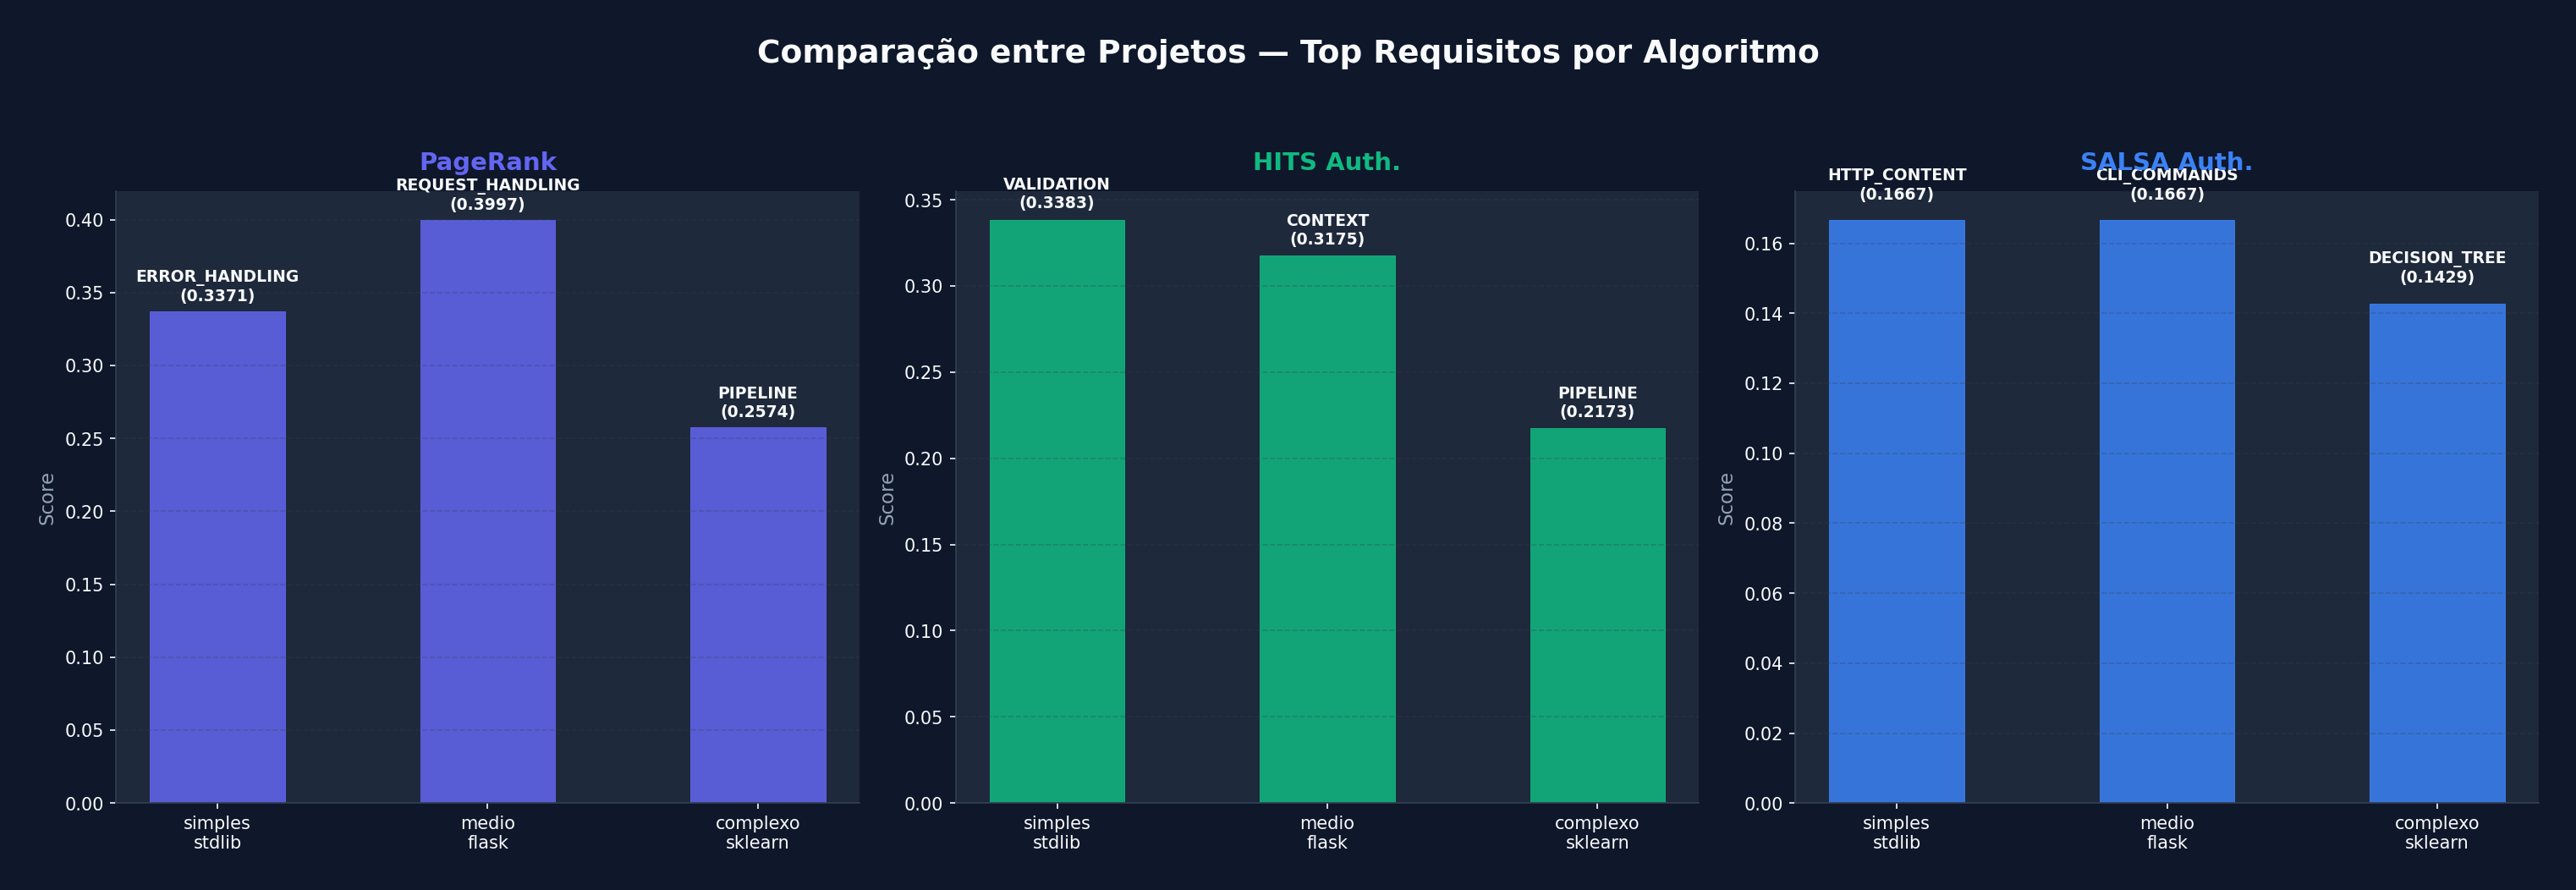
\includegraphics[width=0.95\linewidth]{ranking_comparativo.png}
    \caption{Ranking comparativo entre os três projetos: \emph{top-1}
    por algoritmo em cada caso de estudo. Compare-se com as
    Tabelas~\ref{tab:top3-stdlib}, \ref{tab:top3-flask} e
    \ref{tab:top3-sklearn}.}
    \label{fig:ranking-comparativo}
\end{figure}

% ---------------------------------------------------------------------------
\section{Discussão}
\label{sec:discussao}

A análise cruzada dos resultados quantitativos
(Secção~\ref{sec:res-correlacoes}) e qualitativos
(Secção~\ref{sec:res-rankings}) permite extrair quatro observações
principais:

\begin{enumerate}
    \item \textbf{Concordância parcial, não unanimidade.} Apenas
        dois dos $18$ pares (\emph{stdlib}: PR vs SALSA-auth e
        HITS-hub vs SALSA-hub) satisfazem o critério \emph{a priori}
        de convergência forte. Nos \emph{top-1}, apenas \emph{dois}
        \emph{matches} ocorrem (Flask: PR/HITS-hub em
        \req{REQ\_REQUEST\_HANDLING}; \emph{sklearn}: PR/HITS-auth
        em \req{REQ\_PIPELINE}). A narrativa de ``convergência global
        no caso mais denso'' --- presente em iterações anteriores
        deste trabalho --- não se sustenta face aos coeficientes
        formais.

    \item \textbf{Divergência informativa entre HITS e SALSA versus
        PageRank.} Os pares envolvendo \emph{hubs} (PR vs HITS-hub,
        PR vs SALSA-hub) apresentam correlação muito baixa ou
        ligeiramente negativa em \emph{stdlib} e Flask. Isto confirma
        que \emph{hubs} e \emph{authorities} medem dimensões
        distintas de centralidade --- a \emph{orquestração} é uma
        propriedade dual da \emph{importância transitiva}. Esta
        divergência é \textbf{informativa}, não defeituosa: o
        engenheiro de requisitos pode usar PR para identificar
        ``onde a importância flui'', HITS-auth para identificar
        ``de quem todos dependem'', e HITS-hub para identificar
        ``quem orquestra muitos''.

    \item \textbf{Comportamento do SALSA em grafos pequenos
        --- resultado nulo, não confirmação teórica.}
        O SALSA produziu \emph{distribuições praticamente uniformes}
        em dois dos três casos (Flask e \emph{scikit-learn}). Esta
        observação é consistente com a propriedade demonstrada por
        \citet{lempel2001} --- em grafos não ponderados e fortemente
        conexos, o \emph{score} de \emph{authority} reduz-se a
        $\text{in}(v)/|E|$ ---, mas \textbf{não constitui
        confirmação empírica da mitigação do Efeito TKC}. O Efeito
        TKC pressupõe a existência de \emph{sub-comunidades
        densamente coesas} embutidas em estruturas maiores; nenhum
        dos três grafos analisados apresenta tal característica
        (\cf\ análise estrutural em
        Secção~\ref{sec:res-tec}). Honestamente, este é um
        \emph{resultado nulo}: o SALSA não distinguiu nada onde os
        outros algoritmos distinguiram --- e a vantagem teórica do
        SALSA é \emph{esperada} aparecer em corpora onde o TKC se
        manifesta, condição que o presente corpus não cumpre. A
        propriedade fica assim confirmada apenas no plano teórico
        (Capítulo~\ref{ch:fundamentos}).

    \item \textbf{Acoplamento como propriedade emergente.} Os ciclos
        identificados no Flask e a alta densidade no
        \emph{scikit-learn} não foram inseridos manualmente ---
        emergem do código real. Isto sustenta a tese de que o
        \textbf{grafo de dependências contém informação latente}
        sobre a importância dos requisitos, suficiente para apoiar
        --- mas não substituir --- a decisão dos
        \emph{stakeholders}.
\end{enumerate}

\paragraph{Resposta a RQ3.} A coerência arquitetural dos rankings é
\textbf{moderada e direcionada}: os \emph{top-1} identificados
correspondem a elementos efetivamente centrais nas arquiteturas
conhecidas (a \code{Pipeline} no \emph{scikit-learn} é o coração do
\emph{framework}; o \emph{request handling} no Flask é o
\emph{middleware} central). Contudo, esta correspondência é
\emph{qualitativa} --- baseada na inspeção do investigador, não em
juízo de profissionais externos. A validação humana fica como
trabalho futuro (Secção~\ref{sec:trabalho-futuro}).

\paragraph{Implicações práticas.}
Para um engenheiro de requisitos ou \emph{project manager}
confrontado com um sistema Python existente, os resultados sugerem
um fluxo prático: (1) executar o \emph{ReqGraph} para gerar o grafo
de requisitos; (2) executar o \code{ranker.py} e inspecionar o
\emph{top-5} de cada um dos três algoritmos; (3) considerar
\emph{candidatos a requisito crítico} todos os requisitos que
aparecem no \emph{top-5} de pelo menos dois dos três algoritmos ---
a interseção tem maior probabilidade de captar centralidades
genuínas e menos sensíveis a uma única definição de centralidade.

% ---------------------------------------------------------------------------
\section{Ameaças à Validade}
\label{sec:ameacas}

As ameaças à validade são apresentadas seguindo a taxonomia clássica
de \citet{wohlin2012}, ordenadas por relevância dentro de cada
categoria.

\subsection{Validade de Construto (\emph{Construct Validity})}

\begin{itemize}
    \item \textbf{``Requisito'' como agregação de funções é
        \emph{proxy} discutível.} O artefacto \code{func\_to\_req}
        agrega funções em \emph{domain features} que são
        interpretadas como requisitos. Esta operacionalização não
        coincide com a definição clássica de requisito funcional
        \parencite{sommerville2007}; corresponde antes a uma noção
        de \emph{feature module}. O construto medido é, portanto,
        ``centralidade estrutural de \emph{feature module}'', e não
        ``importância de requisito'' no sentido pleno. Esta
        distinção foi explicitada na nota ontológica
        (Secção~\ref{sec:problema}).

    \item \textbf{Subjetividade deslocada, não eliminada.} A
        priorização estrutural reduz o esforço dos
        \emph{stakeholders}, mas desloca a subjetividade para (a) a
        escolha dos ficheiros analisados e (b) a construção do
        mapeamento \code{func\_to\_req}. A tese
        \emph{não} demonstra que estes dois passos são menos
        subjetivos do que a Votação Acumulativa --- apenas que
        ocorrem em momentos diferentes do processo (\emph{up-front}
        vs.\ \emph{per-requirement}).
\end{itemize}

\subsection{Validade Interna (\emph{Internal Validity})}

\begin{itemize}
    \item \textbf{Ausência de \emph{inter-rater reliability}.} O
        protocolo \code{func\_to\_req}
        (Secção~\ref{sec:protocolo-func2req}) é executado por um
        único investigador. Dois investigadores poderiam produzir
        mapeamentos diferentes, levando a grafos diferentes e a
        rankings potencialmente diferentes. A replicação por um
        segundo investigador, com cálculo de Cohen's $\kappa$, é
        deixada como trabalho futuro.

    \item \textbf{Sensibilidade a parâmetros não testada
        sistematicamente.} O fator de amortecimento do PageRank
        ($d = 0{,}85$) e as tolerâncias de convergência ($10^{-6}$,
        $10^{-8}$) seguem os valores canónicos da literatura. Em
        grafos com $\leq 17$ arestas, a sensibilidade a estes
        parâmetros não é trivial --- uma análise de robustez
        $d \in \{0{,}5, 0{,}7, 0{,}85, 0{,}95\}$ fica registada como
        extensão recomendada.

    \item \textbf{Critério ``a priori'' de convergência protege
        contra \emph{p-hacking}.} A definição em
        Secção~\ref{sec:metricas} foi formulada antes da observação
        dos resultados. Esta opção elimina o risco de o autor
        ajustar o critério \emph{post hoc} para maximizar o número
        de pares ``convergentes''.
\end{itemize}

\subsection{Validade Externa (\emph{External Validity})}

\begin{itemize}
    \item \textbf{Dimensão e diversidade do corpus.} A validação
        assenta em três projetos Python; conclusões sobre a
        generalidade da abordagem a outros ecossistemas (Java, C++,
        TypeScript) requerem extensão futura --- nomeadamente, a
        substituição do \emph{front-end} de AST por outro motor
        (\code{JavaParser}, \code{TypeScript Compiler API} ou
        \code{libclang}).

    \item \textbf{Seleção parcial de ficheiros.} Cada projeto foi
        analisado por meio de uma \emph{amostra} dos seus ficheiros
        (2--4), selecionada como ``\emph{core}''. Esta seleção
        \emph{introduz viés}: requisitos cujas implementações estão
        fora do conjunto selecionado tornam-se \emph{singletons}
        (caso particularmente visível no Flask, com 6 requisitos
        isolados de 13). A replicação sobre o \emph{codebase}
        completo de cada projeto fica como extensão recomendada.

    \item \textbf{Ausência de validação humana.} A coerência
        arquitetural foi avaliada por inspeção do investigador, não
        por engenheiros dos projetos analisados. Esta limitação é
        endereçada na Secção~\ref{sec:trabalho-futuro}.
\end{itemize}

\subsection{Validade de Conclusão (\emph{Conclusion Validity})}

\begin{itemize}
    \item \textbf{Tamanho amostral reduzido para inferências
        estatísticas.} Com $n = 7$ a $9$ vértices, os coeficientes de
        correlação reportados têm intervalos de confiança largos;
        os valores devem ser lidos como \emph{descritivos} dos três
        casos, não como base para inferência sobre uma população de
        projetos.

    \item \textbf{Observação parcial do Efeito TKC.} Os três grafos
        analisados, pela sua pequena dimensão e relativa
        regularidade de graus, não permitem observar o cenário em
        que o SALSA evidenciaria a sua vantagem teórica face ao
        HITS. A conclusão sobre o SALSA é, portanto,
        \emph{honestamente nula}: o algoritmo não distinguiu o que
        os outros distinguiram, e a propriedade teórica não pôde ser
        empiricamente testada neste corpus.

    \item \textbf{Arestas não ponderadas.} Todas as arestas do Grafo
        de Requisitos têm peso unitário. Não é tida em conta a
        frequência de invocação ou a ``força'' semântica do
        acoplamento --- fatores que potencialmente refinariam os
        \emph{scores}.
\end{itemize}

Estas ameaças são endereçadas, sob a forma de propostas de
continuação, na Secção~\ref{sec:trabalho-futuro}.
